\documentclass{dragonfly-report}\usepackage[]{graphicx}\usepackage[]{color}
%% maxwidth is the original width if it is less than linewidth
%% otherwise use linewidth (to make sure the graphics do not exceed the margin)
\makeatletter
\def\maxwidth{ %
  \ifdim\Gin@nat@width>\linewidth
    \linewidth
  \else
    \Gin@nat@width
  \fi
}
\makeatother

\definecolor{fgcolor}{rgb}{0.345, 0.345, 0.345}
\newcommand{\hlnum}[1]{\textcolor[rgb]{0.686,0.059,0.569}{#1}}%
\newcommand{\hlstr}[1]{\textcolor[rgb]{0.192,0.494,0.8}{#1}}%
\newcommand{\hlcom}[1]{\textcolor[rgb]{0.678,0.584,0.686}{\textit{#1}}}%
\newcommand{\hlopt}[1]{\textcolor[rgb]{0,0,0}{#1}}%
\newcommand{\hlstd}[1]{\textcolor[rgb]{0.345,0.345,0.345}{#1}}%
\newcommand{\hlkwa}[1]{\textcolor[rgb]{0.161,0.373,0.58}{\textbf{#1}}}%
\newcommand{\hlkwb}[1]{\textcolor[rgb]{0.69,0.353,0.396}{#1}}%
\newcommand{\hlkwc}[1]{\textcolor[rgb]{0.333,0.667,0.333}{#1}}%
\newcommand{\hlkwd}[1]{\textcolor[rgb]{0.737,0.353,0.396}{\textbf{#1}}}%

\usepackage{framed}
\makeatletter
\newenvironment{kframe}{%
 \def\at@end@of@kframe{}%
 \ifinner\ifhmode%
  \def\at@end@of@kframe{\end{minipage}}%
  \begin{minipage}{\columnwidth}%
 \fi\fi%
 \def\FrameCommand##1{\hskip\@totalleftmargin \hskip-\fboxsep
 \colorbox{shadecolor}{##1}\hskip-\fboxsep
     % There is no \\@totalrightmargin, so:
     \hskip-\linewidth \hskip-\@totalleftmargin \hskip\columnwidth}%
 \MakeFramed {\advance\hsize-\width
   \@totalleftmargin\z@ \linewidth\hsize
   \@setminipage}}%
 {\par\unskip\endMakeFramed%
 \at@end@of@kframe}
\makeatother

\definecolor{shadecolor}{rgb}{.97, .97, .97}
\definecolor{messagecolor}{rgb}{0, 0, 0}
\definecolor{warningcolor}{rgb}{1, 0, 1}
\definecolor{errorcolor}{rgb}{1, 0, 0}
\newenvironment{knitrout}{}{} % an empty environment to be redefined in TeX

\usepackage{alltt}
%\documentclass{article}

\usepackage{hyperref}
\usepackage{subfig}

\title{Improving steepness priors in \emph{fishnets}}{Improving
  priors for the steepness of the stock-recruitment function within the R package \emph{fishnets}}

\subtitle{}
\author{Philipp Neubauer}

\addbibresource{steepness.bib}
\IfFileExists{upquote.sty}{\usepackage{upquote}}{}
\begin{document}
\maketitle

\section{Inferring steepness: available literature and estimation in the context of fishnets}

Steepness is generally defined as the fraction of recruitment from an unfished population ($R_0$) when the spawning stock biomass is at 20\% of its unfished (equilibrium) level ($B_0$). Given a functional form of the stock-recruit function $f$, steepness can be tied to the parameters of that function (at least in the case of the Ricker and Beverton-Holt (B-H) S-R functions), such that parameters of $f$ can be expressed in terms of steepness. However, depending on the form of $f$, the bounds on steepness are different: the Beverton-Holt S-R function admits steepness values in $[0.2;1]$ while the Ricker S-R function admits values between $0.2$ and infinity (i.e., recruitment can increase above $R_0$ at $0.2 B_0$). 

Theory provides some insight into potential life history predictors for steepness. For example, recruitment variability and natural mortality M set the lower bounds for steepness \citep{he_2006_prior}. However, at low recruitment variability and M, there is little information about steepness in these parameters alone. Given an age structured model, Mangel et al. (2010; 2013) showed that steepness depends on growth, fecundity and (larval and adult) mortality rates, and \citet{rose2001compensatory} provided evidence that empirical estimates of steepness follow expectations from life-history theory. However, given the multitude of assumptions that need to be made for a node based on theory alone (i.e., the Mangel et al. model), from larval mortality schedules to fecundity at age, a theoretical node was deemed achievable in the context of fishnets. As an aside, the Mangel et al. paper should be understood as an exercise that provides a mechanistic underpinning for steepness, not a practically applicable model. 

The most promising avenue for a steepness node within fishnets that could be used to predict steepness for (almost) arbitrary stocks, seemed an empirical node that relates steepness to life-history. The biggest issue with the empirical node, however, was that the somewhat outdated and biased (see below) \citet{myers_1999_maximum} remains the only data source that spans a range of families and orders. \citet{shertzer2012spawner} obtained priors for demersal fish, but only provided an ad-hoc fit of truncated normal and beta distributions to estimates of steepness from stock assessments (for south-east US stocks only). They did not provide individual estimates for species. Other datasets that provide more formally derived (and unbiased) priors for steepness (e.g., \citet{michielsens_2004_bayesian}, \citet{dorn2002advice} and \citet{forrest2010hierarchical}) are too narrow to inform over broad enough a taxonomic range for an empirical node.

Given that the range of steepness varies among the B-H and Ricker S-R functions, steepness estimated from one S-R function is not directly applicable to the other. This posed a non-trivial problem for the development of a general purpose prior for steepness; Ideally, the steepness node should have a method for Ricker and B-H steepness. However, empirical approaches to the specification of prior distributions for steepness have generally focused on either one S-R model (with \citet{michielsens_2004_bayesian} and \citet{forrest2010hierarchical} being the exceptions). \citet{myers_1999_maximum} first provided estimates of B-H steepness for a large number of species and families based on Myers' S-R database. The estimates were simple transformations of the maximum lifetime reproductive rate, which was estimated from a meta-analysis using the Ricker S-R model across all stocks. \citet{michielsens_2004_bayesian} pointed out that fits of the Ricker and B-H functions lead to different estimates for the slope at the origin and different expectations for steepness. The direct transformation from Ricker model parameters to B-H steepness applied in Myers et al. 1999 therefore gives misleading (i.e., overly conservative) results. Furthermore, there is a potentially strong selection bias in the study (for managed, VPA assessed stocks), which could have further biased results at species level by including only a biased subset of populations for any particular species.

Nevertheless, short of doing a new meta-analysis of steepness from the RAM legacy DB or other data source, \citet{myers_1999_maximum} was considered the only possible starting point for an empirical node in fishnets. Estimates for US/Canada west-coast rockfish from \citet{forrest2010hierarchical} were included to improve estimates of empirical relationships with life-history parameters, as were estimates for tuna by S. Harley from \url{https://www.wcpfc.int/system/files/SC-7-SA-WP-04\%20\%5BSKJ\%20Assessment-rev1\%5D.pdf}. The reported estimates for the maximum lifetime reproductive rate in \citet{myers_1999_maximum} made it possible to re-calculate the Ricker steepness (alongside the somewhat biased Beverton-Holt steepness reported in their paper). These estimates were then combined with life-history information in fishbase to build a predictive model for steepness within fishnets. Given the complex relationships between life-history parameters and their constraints on steepness, a non-parametric node based on `brter` was considered the most practical starting point.

\section{An empirical steepness node}

\subsection{Data: a collated dataset for steepness}

Empirical estimates based on maximum lifetime reproductive rates were extracted from \citet{myers_1999_maximum}, and both mean B-H and Ricker steepness were recorded (the latter calculated using formulae in \citet{michielsens_2004_bayesian}), along with other parameters reported in \citet{myers_1999_maximum}. These data were augmented with data from \citet{forrest2010hierarchical} for \emph{Sebastes ssp.} and estimates from S. Harley for tuna. The combined dataset is available in the $\/data\/steepness$ directory as Myers\_et\_al\_steepness\_extended.csv. Data at the family level was also extracted and saved into Myers\_et\_al\_steepness\_families\_extended.csv.




A data node for steepness was implemented, such that 
\begin{knitrout}
\definecolor{shadecolor}{rgb}{0.969, 0.969, 0.969}\color{fgcolor}\begin{kframe}
\begin{alltt}
\hlcom{# Source in the package ----}

\hlkwd{source}\hlstd{(}\hlstr{'collate.R'}\hlstd{)}
\hlkwd{require}\hlstd{(dplyr)}

\hlstd{steep} \hlkwb{<-} \hlstd{Steepness}\hlopt{$}\hlkwd{create}\hlstd{(}\hlstr{'./data/steepness'}\hlstd{)}
\hlkwd{head}\hlstd{(}\hlkwd{tbl_df}\hlstd{(steep))}
\end{alltt}
\begin{verbatim}
## Source: local data frame [6 x 11]
## 
##                species populations
## 1    Harpodon nehereus           1
## 2 Alosa pseudoharengus           4
## 3    Alosa sapidissima           1
## 4  Brevoortia tyrannus           1
## 5     Alosa aestivalis           3
## 6  Brevoortia patronus           1
## Variables not shown: log_alpha_tilde (dbl),
##   SE_log_alpha_tilde (dbl), var_log_alpha_tilde
##   (dbl), exp_alpha_hat (dbl), z_20 (dbl), z_50
##   (dbl), z_80 (dbl), mean_R_z (dbl), mean_BH_z
##   (dbl)
\end{verbatim}
\end{kframe}
\end{knitrout}

returns the data table. The table can then be merged with a fishbase data extract to pair empirical steepness estimates with life-history data. Note that the fishbase data is not restricted to species with $z$ estimates, rather the merge is, in SQL terms, a left join onto the fishbase data:

\begin{knitrout}
\definecolor{shadecolor}{rgb}{0.969, 0.969, 0.969}\color{fgcolor}\begin{kframe}
\begin{alltt}
\hlcom{# Load the Fishbase data}
\hlstd{fb} \hlkwb{<-} \hlstd{FishbaseWeb}\hlopt{$}\hlkwd{read}\hlstd{(}\hlstr{'data/fishbase-web'}\hlstd{)}
\hlcom{# Limit to the 7940 with both k and linf}
\hlstd{fb} \hlkwb{<-} \hlkwd{subset}\hlstd{(fb,}\hlopt{!}\hlkwd{is.na}\hlstd{(k)} \hlopt{& !}\hlkwd{is.na}\hlstd{(linf))}
\hlcom{# An an id column for indexing later}
\hlstd{fb}\hlopt{$}\hlstd{id} \hlkwb{<-} \hlnum{1}\hlopt{:}\hlkwd{nrow}\hlstd{(fb)}
\hlcom{# Add a dummy row for helping with predictor nodes}
\hlcom{# that need to have at least two predictors}
\hlstd{fb}\hlopt{$}\hlstd{dummy} \hlkwb{<-} \hlnum{1.0}

\hlcom{# merge with steepness data}
\hlstd{steep_merged} \hlkwb{<-} \hlstd{Steepness}\hlopt{$}\hlkwd{merge}\hlstd{(steep,fb)}

\hlkwd{head}\hlstd{(}\hlkwd{tbl_df}\hlstd{(steep_merged))}
\end{alltt}
\begin{verbatim}
## Source: local data frame [6 x 46]
## 
##               species populations log_alpha_tilde
## 1 Abbottina rivularis          NA              NA
## 2      Ablennes hians          NA              NA
## 3       Abramis brama          NA              NA
## 4       Abramis brama          NA              NA
## 5       Abramis brama          NA              NA
## 6       Abramis brama          NA              NA
## Variables not shown: SE_log_alpha_tilde (dbl),
##   var_log_alpha_tilde (dbl), exp_alpha_hat (dbl),
##   z_20 (dbl), z_50 (dbl), z_80 (dbl), mean_R_z
##   (dbl), mean_BH_z (dbl), order (fctr), country
##   (fctr), sex (fctr), genus (fctr), family
##   (fctr), swimmode (fctr), ltype (fctr), linf
##   (dbl), k (dbl), t0 (dbl), m (dbl), temp (dbl),
##   lmat (dbl), lmatmin (dbl), lmatmax (dbl), amat
##   (dbl), amatmin (dbl), amatmax (dbl), a (dbl), b
##   (dbl), trophic (dbl), diet (fctr), feeding
##   (fctr), habit (fctr), migration (fctr),
##   depthmin (dbl), depthmax (dbl), fecundmin
##   (dbl), fecundmax (dbl), fecundity (dbl), class
##   (fctr), lmax (dbl), amax (dbl), id (int), dummy
##   (dbl)
\end{verbatim}
\end{kframe}
\end{knitrout}

In order to set up a fishnet that that extracts empirical relationships between steepness and life-history, the merged fishbase/steepness data was aggregated at species level to avoid multiple, possibly contradictory, life-history correlates with steepness. Geometric means were used to aggregate life-history parameters, under the assumption that most follow log-normal distributions.

\begin{knitrout}
\definecolor{shadecolor}{rgb}{0.969, 0.969, 0.969}\color{fgcolor}\begin{kframe}
\begin{alltt}
\hlcom{# geometric mean}
\hlstd{gmean} \hlkwb{<-} \hlkwa{function}\hlstd{(}\hlkwc{x}\hlstd{)} \hlkwd{exp}\hlstd{(}\hlkwd{mean}\hlstd{(}\hlkwd{log}\hlstd{(x),}\hlkwc{na.rm}\hlstd{=T))}

\hlcom{# reduce dataset; gometric means for paramters by species}
\hlstd{steep_reduced} \hlkwb{<-} \hlstd{steep_merged} \hlopt
  \hlkwd{select}\hlstd{(species,}
         \hlstd{genus,}
         \hlstd{family,}
         \hlstd{class,}
         \hlstd{order,}
         \hlstd{mean_BH_z,}
         \hlstd{linf,}
         \hlstd{m,}
         \hlstd{fecundity,}
         \hlstd{trophic,}
         \hlstd{lmat,}
         \hlstd{lmax ,}
         \hlstd{k,}
         \hlstd{amax,}
         \hlstd{habit,}
         \hlstd{trophic,}
         \hlstd{depthmax)} \hlopt
  \hlkwd{group_by}\hlstd{(order,class,genus,family,species)} \hlopt
  \hlkwd{summarise}\hlstd{(}\hlkwc{mean_BH_z} \hlstd{=} \hlkwd{unique}\hlstd{(mean_BH_z),}
            \hlkwc{habit} \hlstd{=} \hlkwd{unique}\hlstd{(habit),}
            \hlkwc{trophic} \hlstd{=} \hlkwd{gmean}\hlstd{(trophic),}
            \hlkwc{linf} \hlstd{=} \hlkwd{gmean}\hlstd{(linf),}
            \hlkwc{m} \hlstd{=} \hlkwd{gmean}\hlstd{(m),}
            \hlkwc{depthmax} \hlstd{=} \hlkwd{gmean}\hlstd{(depthmax),}
            \hlkwc{fecundity} \hlstd{=} \hlkwd{gmean}\hlstd{(fecundity),}
            \hlkwc{trophic} \hlstd{=} \hlkwd{gmean}\hlstd{(trophic),}
            \hlkwc{lmax} \hlstd{=} \hlkwd{gmean}\hlstd{(lmax),}
            \hlkwc{lmat} \hlstd{=} \hlkwd{gmean}\hlstd{(lmat),}
            \hlkwc{k} \hlstd{=} \hlkwd{gmean}\hlstd{(k),}
            \hlkwc{amax} \hlstd{=} \hlkwd{gmean}\hlstd{(amax),}
            \hlkwc{recsigma} \hlstd{=} \hlnum{NA}\hlstd{)} \hlopt
  \hlkwd{ungroup}\hlstd{()} \hlopt
  \hlkwd{data.frame}\hlstd{()}
\end{alltt}
\end{kframe}
\end{knitrout}

\subsection{A Bayesian empirical node to avoid over-fitting}

An initial attempt at defining a fishnet based on previously available nodes (Brter: boosted regression trees; Svmer: support vector machines; Glmer: generalized linear models) suggested that over-fitting of empirical relationships might be interfering with predictive power of the nodes. To investigate this potential problem, I implemented a Bayesian node based on the \href{http://www.r-inla.org/}{INLA} package in R. Fully Bayesian methods are less prone to over-fitting, and the INLA approach, based on Laplacian approximations, allows for fast parameter estimation in linear and linear mixed models. The resulting node, called \emph{Bayser}, uses the same formula syntax as previous empirical nodes, with additional option to estimate random effects with the $f(effect, 'iid')$ syntax (e.g., f(family,model="iid") for a family level random effect). This option should facilitate the use of taxonomic information in empirical nodes, whereas the use of taxonomy as a fixed effect frequently leads to over-fitting. The \emph{Bayser} node comes with $fit$, $sample$, $predict$ and $tune$ methods:

\begin{knitrout}
\definecolor{shadecolor}{rgb}{0.969, 0.969, 0.969}\color{fgcolor}\begin{kframe}
\begin{alltt}
\hlstd{linf} \hlkwb{=} \hlkwd{Bayser}\hlstd{(}\hlkwd{log}\hlstd{(linf)} \hlopt{~} \hlkwd{f}\hlstd{(family,}\hlkwc{model}\hlstd{=}\hlstr{"iid"}\hlstd{)} \hlopt{+}
                \hlkwd{f}\hlstd{(order,}\hlkwc{model}\hlstd{=}\hlstr{"iid"}\hlstd{)} \hlopt{+}
                \hlkwd{log}\hlstd{(lmax)} \hlopt{+}
                \hlstd{habit,exp)}

\hlcom{# fitting to data}
\hlstd{linf}\hlopt{$}\hlkwd{fit}\hlstd{(steep_reduced[}\hlnum{1}\hlopt{:}\hlnum{1500}\hlstd{,])}
\hlstd{psamp} \hlkwb{<-} \hlnum{1501}\hlopt{:}\hlkwd{nrow}\hlstd{(steep_reduced)}

\hlcom{# predicting onto new data}
\hlstd{example_predictions} \hlkwb{<-} \hlstd{linf}\hlopt{$}\hlkwd{predict}\hlstd{(steep_reduced[psamp,])}

\hlstd{nna_data} \hlkwb{<-} \hlopt{!}\hlkwd{is.na}\hlstd{(steep_reduced}\hlopt{$}\hlstd{lmax[psamp])}

\hlstd{predict_df} \hlkwb{<-} \hlkwd{data.frame}\hlstd{(}\hlkwc{bayser} \hlstd{= example_predictions[nna_data],}
                         \hlkwc{observed} \hlstd{= steep_reduced[psamp,}\hlstr{'linf'}\hlstd{][nna_data])}

\hlstd{linf_brter} \hlkwb{=} \hlkwd{Brter}\hlstd{(}\hlkwd{log}\hlstd{(linf)} \hlopt{~} \hlstd{family} \hlopt{+}
                     \hlstd{order} \hlopt{+}
                     \hlkwd{log}\hlstd{(lmax)} \hlopt{+}
                     \hlstd{habit,exp)}

\hlcom{# fitting to data}
\hlstd{linf_brter}\hlopt{$}\hlkwd{fit}\hlstd{(steep_reduced[}\hlnum{1}\hlopt{:}\hlnum{1500}\hlstd{,])}
\end{alltt}
\begin{verbatim}
## [1] fitting gbm model with a fixed number of 2000 trees for log(linf)
## [1] total deviance = 228.52
## [1] residual deviance = 19.84
## predictors: family order log(lmax) habit
\end{verbatim}
\begin{alltt}
\hlcom{# predicting onto new data}
\hlstd{example_predictions_brter} \hlkwb{<-} \hlstd{linf_brter}\hlopt{$}\hlkwd{predict}\hlstd{(steep_reduced[psamp,])}

\hlstd{predict_df} \hlkwb{<-} \hlstd{reshape2}\hlopt{::}\hlkwd{melt}\hlstd{(}\hlkwd{data.frame}\hlstd{(}\hlkwc{brter} \hlstd{= example_predictions_brter[nna_data],}
                                        \hlstd{predict_df),}
                             \hlkwc{id.vars} \hlstd{=} \hlkwd{c}\hlstd{(}\hlstr{'observed'}\hlstd{))}
\end{alltt}
\end{kframe}
\end{knitrout}

\begin{knitrout}
\definecolor{shadecolor}{rgb}{0.969, 0.969, 0.969}\color{fgcolor}\begin{kframe}
\begin{alltt}
\hlkwd{require}\hlstd{(ggplot2)}

\hlkwd{ggplot}\hlstd{(predict_df)} \hlopt{+}
  \hlkwd{geom_point}\hlstd{(}\hlkwd{aes}\hlstd{(}\hlkwc{y} \hlstd{= value,} \hlkwc{x} \hlstd{= observed,} \hlkwc{col} \hlstd{= variable))} \hlopt{+}
  \hlkwd{geom_abline}\hlstd{(}\hlkwc{slope}\hlstd{=}\hlnum{1}\hlstd{,} \hlkwc{intercept}\hlstd{=}\hlnum{0}\hlstd{)} \hlopt{+}
  \hlkwd{theme_bw}\hlstd{()} \hlopt{+}
  \hlkwd{xlab}\hlstd{(}\hlstr{'Data'}\hlstd{)} \hlopt{+}
  \hlkwd{ylab}\hlstd{(}\hlstr{'Prediction'}\hlstd{)} \hlopt{+}
  \hlkwd{scale_colour_discrete}\hlstd{(}\hlstr{'Method'}\hlstd{)}
\end{alltt}
\end{kframe}\begin{figure}
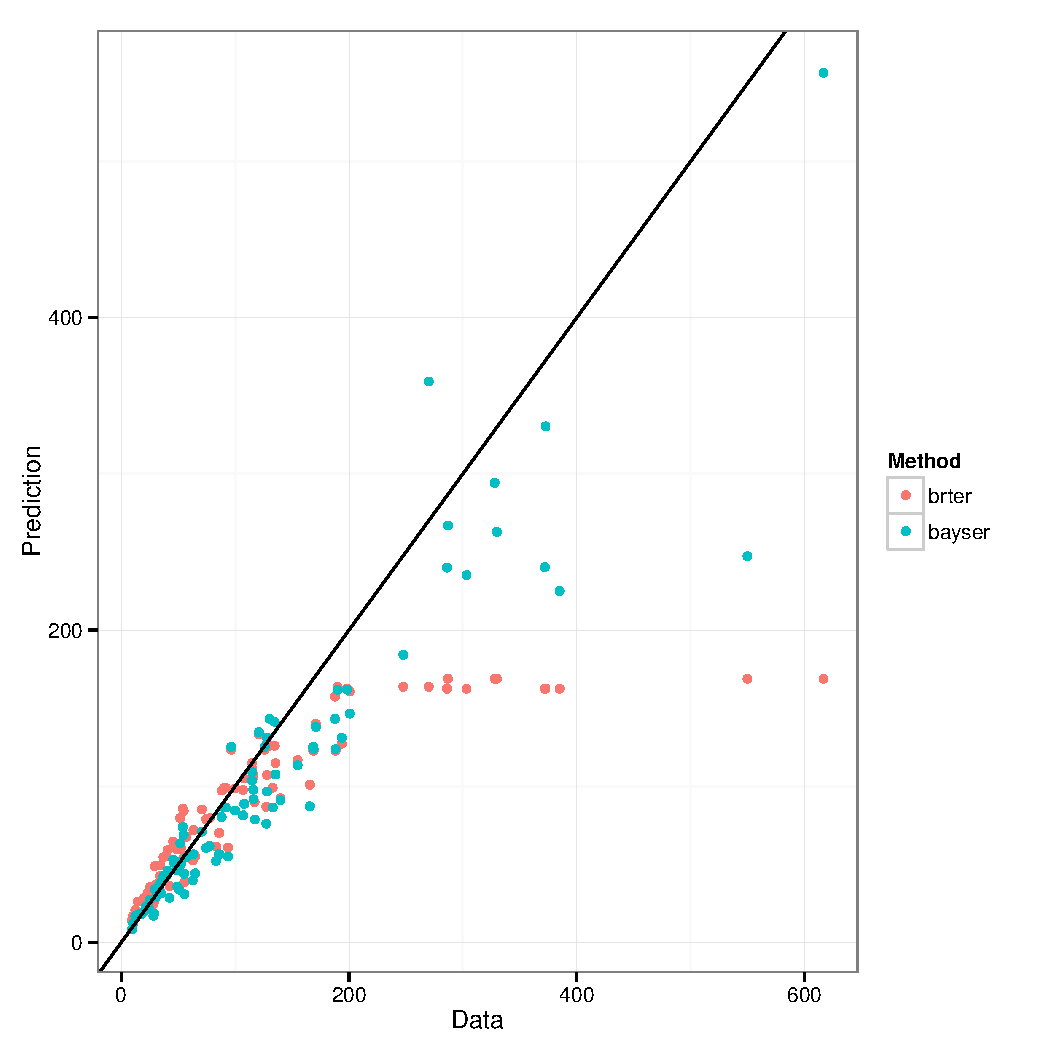
\includegraphics[width=\maxwidth]{figure/unnamed-chunk-2-1} \caption[Example predictions for linf as a function of lmax and taxonomy on a subset of fishbase data, showing that the predictive power in Bayser can be superior to that of Brter when taxonomy is used as a predictor]{Example predictions for linf as a function of lmax and taxonomy on a subset of fishbase data, showing that the predictive power in Bayser can be superior to that of Brter when taxonomy is used as a predictor.\label{fig:unnamed-chunk-2}}
\end{figure}


\end{knitrout}


\subsection{Sequential imputing of data in fishnets}

In the $Bayser$ example above, $linf$ depends on $lmax$ in an empirical node. The relationship can only be estimated for data rows (i.e.,species) with data for both traits. For more complex life history interactions, missing data for the combination of covariates in the model can strongly influence the total number of species for which the relationship can be striated. For example, one species may not have a reported von Bertlanaffy k, while another species may have k but no estimate of fecundity. Neither row could be included in a node like steepness, which may depend on both factors. In the case of steepness, only 46 empirical estimates at the species level are available from the dataset described above, and missing values dramatically reduce the number of covariates that could be used to construct an empirical node for steepness.

To obtain more data for complex empirical relationships, I implemented an option within the generic $fit$ method of a fishnet, which allows data to be sequentially imputed. Thus, if linf depends on lmax, and k in turn depends on linf, then linf could be imputed for species with missing linf based on the node relating it to lmax. This allows k to be estimated for species with data for lamx and missing data for linf. The imputation naturally relies on a linearly evolving net, where relationships depend on  values imputed at lower level nodes. The option can be turned on using $impute = TRUE$ when fitting a fishnet (see the steepness node fitting below).

\subsection{The empirical steepness node: fishing for predictive power}

The empirical fishnet node to estimate steepness was embedded in a larger fishnet that aimed to build a covariate set (using the $impute~=~T$ option). All empirical nodes leading up to steepness node itself used the Bayser node, and included taxonomic information as random effects. The actual steepness node was initially specified as a $Brter$ node, in order to capture potentially non-linear relationships between steepness and co-variates. After some discussion, the B-H estimates from Myers et all were used as these were deemed most useful in the context of NZ stock assessments, which seem to overwhelmingly use B-H S-R functions.

\begin{knitrout}
\definecolor{shadecolor}{rgb}{0.969, 0.969, 0.969}\color{fgcolor}\begin{kframe}
\begin{alltt}
\hlcom{# build a net for steepnes. }
\hlcom{# Use Bayesian nodes in an attempt to not overfit}
\hlcom{# Transformations are defined for Beverton-Holt S-R }
\hlcom{# parameters to map steepness onto the real line and back.}

\hlstd{logit} \hlkwb{<-} \hlkwa{function}\hlstd{(}\hlkwc{x}\hlstd{)} \hlkwd{log}\hlstd{(x}\hlopt{/}\hlstd{(}\hlnum{1}\hlopt{-}\hlstd{x))}
\hlstd{logit_inv} \hlkwb{<-} \hlkwa{function}\hlstd{(}\hlkwc{xt}\hlstd{)} \hlnum{1}\hlopt{/}\hlstd{(}\hlnum{1} \hlopt{+} \hlkwd{exp}\hlstd{(}\hlopt{-}\hlstd{xt))}
\hlstd{BH_tr} \hlkwb{<-} \hlkwa{function}\hlstd{(}\hlkwc{h}\hlstd{) h}\hlopt{/}\hlnum{0.8}\hlopt{-}\hlnum{0.25}
\hlstd{BH_tr_inv} \hlkwb{<-} \hlkwa{function}\hlstd{(}\hlkwc{ht}\hlstd{) (ht}\hlopt{+}\hlnum{0.25}\hlstd{)}\hlopt{*}\hlnum{0.8}
\hlstd{logit_BH} \hlkwb{<-} \hlkwa{function}\hlstd{(}\hlkwc{h}\hlstd{)} \hlkwd{logit}\hlstd{(}\hlkwd{BH_tr}\hlstd{(h))}
\hlstd{logit_BH_inv} \hlkwb{<-} \hlkwa{function}\hlstd{(}\hlkwc{ht}\hlstd{)} \hlkwd{BH_tr_inv}\hlstd{(}\hlkwd{logit_inv}\hlstd{(ht))}

\hlstd{BH_net} \hlkwb{<-} \hlkwd{Fishnet}\hlstd{(}
  \hlkwc{species}   \hlstd{=} \hlkwd{SpeciesRandom}\hlstd{(),}
  \hlkwc{genus}     \hlstd{=} \hlkwd{GenusParser}\hlstd{(),}
  \hlkwc{family}    \hlstd{=} \hlkwd{FamilyLookupper}\hlstd{(),}
  \hlkwc{order}     \hlstd{=} \hlkwd{OrderLookupper}\hlstd{(),}
  \hlkwc{class}     \hlstd{=} \hlkwd{ClassLookupper}\hlstd{(),}

  \hlkwc{habit}     \hlstd{=} \hlkwd{TaxonomicImputer}\hlstd{(}\hlstr{'habit'}\hlstd{),}
  \hlkwc{depthmax}  \hlstd{=} \hlkwd{TaxonomicImputer}\hlstd{(}\hlstr{'depthmax'}\hlstd{,}\hlkwd{c}\hlstd{(log,exp),}\hlnum{5}\hlstd{),}
  \hlkwc{trophic}   \hlstd{=} \hlkwd{TaxonomicImputer}\hlstd{(}\hlstr{'trophic'}\hlstd{,}\hlkwd{c}\hlstd{(log,exp),}\hlnum{3}\hlstd{),}
  \hlkwc{lmax}      \hlstd{=} \hlkwd{TaxonomicImputer}\hlstd{(}\hlstr{'lmax'}\hlstd{,}\hlkwd{c}\hlstd{(log,exp),}\hlnum{5}\hlstd{),}
  \hlkwc{amax}      \hlstd{=} \hlkwd{TaxonomicImputer}\hlstd{(}\hlstr{'amax'}\hlstd{,}\hlkwd{c}\hlstd{(log,exp),}\hlnum{5}\hlstd{),}

  \hlkwc{linf}      \hlstd{=} \hlkwd{Bayser}\hlstd{(}\hlkwd{log}\hlstd{(linf)} \hlopt{~} \hlkwd{f}\hlstd{(family,}\hlkwc{model}\hlstd{=}\hlstr{"iid"}\hlstd{)} \hlopt{+}
                       \hlkwd{f}\hlstd{(class,}\hlkwc{model}\hlstd{=}\hlstr{"iid"}\hlstd{)} \hlopt{+}
                       \hlkwd{log}\hlstd{(lmax),exp),}

  \hlkwc{fecundity} \hlstd{=} \hlkwd{Bayser}\hlstd{(}\hlkwd{log}\hlstd{(fecundity)} \hlopt{~} \hlkwd{f}\hlstd{(family,}\hlkwc{model}\hlstd{=}\hlstr{"iid"}\hlstd{)} \hlopt{+}
                       \hlkwd{f}\hlstd{(class,}\hlkwc{model}\hlstd{=}\hlstr{"iid"}\hlstd{)} \hlopt{+}
                       \hlkwd{log}\hlstd{(linf)} \hlopt{+}
                       \hlkwd{log}\hlstd{(depthmax),exp),}

  \hlkwc{k}         \hlstd{=} \hlkwd{Bayser}\hlstd{(}\hlkwd{log}\hlstd{(k)} \hlopt{~} \hlkwd{f}\hlstd{(family,}\hlkwc{model}\hlstd{=}\hlstr{"iid"}\hlstd{)} \hlopt{+}
                       \hlkwd{log}\hlstd{(linf)} \hlopt{+}
                       \hlkwd{f}\hlstd{(habit,}\hlkwc{model}\hlstd{=}\hlstr{"iid"}\hlstd{)} \hlopt{+}
                       \hlkwd{log}\hlstd{(depthmax),exp),}

  \hlkwc{m}         \hlstd{=} \hlkwd{Bayser}\hlstd{(}\hlkwd{log}\hlstd{(m)} \hlopt{~} \hlkwd{f}\hlstd{(family,}\hlkwc{model}\hlstd{=}\hlstr{"iid"}\hlstd{)} \hlopt{+}
                       \hlkwd{f}\hlstd{(class,}\hlkwc{model}\hlstd{=}\hlstr{"iid"}\hlstd{)} \hlopt{+}
                       \hlkwd{log}\hlstd{(k)} \hlopt{+}
                       \hlkwd{log}\hlstd{(linf)} \hlopt{+}
                       \hlkwd{f}\hlstd{(habit,}\hlkwc{model}\hlstd{=}\hlstr{"iid"}\hlstd{)} \hlopt{+}
                       \hlkwd{log}\hlstd{(depthmax)} \hlopt{+}
                       \hlstd{trophic,exp),}

  \hlkwc{lmat}      \hlstd{=} \hlkwd{Bayser}\hlstd{(}\hlkwd{log}\hlstd{(lmat)} \hlopt{~} \hlkwd{f}\hlstd{(family,}\hlkwc{model}\hlstd{=}\hlstr{"iid"}\hlstd{)} \hlopt{+}
                       \hlkwd{log}\hlstd{(k)} \hlopt{+}
                       \hlkwd{log}\hlstd{(linf)} \hlopt{+}
                       \hlkwd{f}\hlstd{(habit,}\hlkwc{model}\hlstd{=}\hlstr{"iid"}\hlstd{)} \hlopt{+}
                       \hlkwd{log}\hlstd{(depthmax),exp),}

  \hlkwc{recsigma}  \hlstd{=} \hlkwd{RecsigmaThorsonEtAl2014}\hlstd{(),}

  \hlkwc{mean_BH_z} \hlstd{=} \hlkwd{Brter}\hlstd{(}\hlkwd{logit_BH}\hlstd{(mean_BH_z)} \hlopt{~}  \hlstd{habit} \hlopt{+}
                      \hlkwd{log}\hlstd{(linf)} \hlopt{+}
                      \hlkwd{log}\hlstd{(k)} \hlopt{+}
                      \hlkwd{log}\hlstd{(m)} \hlopt{+}
                      \hlkwd{log}\hlstd{(fecundity)} \hlopt{+}
                      \hlstd{recsigma} \hlopt{+}
                      \hlstd{trophic} \hlopt{+}
                      \hlkwd{log}\hlstd{(depthmax),}
                    \hlkwc{transform} \hlstd{= logit_BH_inv,}
                    \hlkwc{ntrees} \hlstd{=}\hlnum{3500}\hlstd{,}
                    \hlkwc{bag.fraction}\hlstd{=}\hlnum{0.9}\hlstd{)}

\hlstd{)}

\hlcom{# fit the BH_et to the summarised fishbase data}
\hlstd{BH_net}\hlopt{$}\hlkwd{fit}\hlstd{(steep_reduced,}\hlkwc{impute} \hlstd{= T)}
\end{alltt}
\end{kframe}
\end{knitrout}

The predictive power of the steepness node was assessed using jackknifing and a newly implemented tune method for Brter. The tune formulation included 6 formulae with increasing amounts of life-history information.

\begin{knitrout}
\definecolor{shadecolor}{rgb}{0.969, 0.969, 0.969}\color{fgcolor}\begin{kframe}
\begin{alltt}
\hlcom{# function to make testset for cross validation}
\hlstd{make_testset} \hlkwb{<-} \hlkwa{function}\hlstd{(}\hlkwc{net}\hlstd{,}\hlkwc{org_data}\hlstd{,}\hlkwc{name}\hlstd{)\{}
  \hlstd{testset} \hlkwb{<-} \hlkwd{data.frame}\hlstd{(net}\hlopt{$}\hlstd{data[,}\hlopt{-}\hlkwd{which}\hlstd{(}\hlkwd{colnames}\hlstd{(net}\hlopt{$}\hlstd{data)} \hlopt{==} \hlstd{name)],}
                        \hlkwc{name} \hlstd{= org_data[name])}
  \hlstd{testset}
\hlstd{\}}

\hlstd{testset} \hlkwb{<-} \hlkwd{make_testset}\hlstd{(BH_net,steep_reduced,}\hlstr{'mean_BH_z'}\hlstd{)}

\hlcom{# jacknifing - could be done with $cross, }
\hlcom{# but is implemented here to produce }
\hlcom{# a vector of observed and predicted outcomes.}

\hlstd{jackknife_cv} \hlkwb{<-} \hlkwa{function}\hlstd{(}\hlkwc{data}\hlstd{,}\hlkwc{net}\hlstd{,}\hlkwc{node}\hlstd{)\{}
  \hlstd{testnet} \hlkwb{<-} \hlstd{net}
  \hlstd{data} \hlkwb{=} \hlstd{data[}\hlopt{!}\hlkwd{is.na}\hlstd{(data[[node]]),]}

  \hlstd{pred} \hlkwb{<-} \hlkwd{vector}\hlstd{(,}\hlkwd{nrow}\hlstd{(data))}
  \hlkwa{for} \hlstd{(i} \hlkwa{in} \hlnum{1}\hlopt{:}\hlkwd{nrow}\hlstd{(data))\{}
    \hlkwd{cat}\hlstd{(}\hlstr{'CV for observation '}\hlstd{,i,}\hlstr{'\textbackslash{}n'}\hlstd{)}
    \hlstd{train} \hlkwb{<-} \hlstd{data[}\hlopt{-}\hlstd{i,]}
    \hlstd{test} \hlkwb{<-} \hlstd{data[i,]}
    \hlstd{test[[node]]} \hlkwb{<-} \hlnum{NA}
    \hlstd{testnet}\hlopt{$}\hlstd{nodes[[node]]}\hlopt{$}\hlkwd{fit}\hlstd{(train)}
    \hlstd{pred[i]} \hlkwb{<-} \hlstd{testnet}\hlopt{$}\hlstd{nodes[[node]]}\hlopt{$}\hlkwd{predict}\hlstd{(test)}

  \hlstd{\}}
  \hlkwd{data.frame}\hlstd{(}\hlkwc{Predicted} \hlstd{= pred,}\hlkwc{Observed} \hlstd{= data[[node]])}
\hlstd{\}}

\hlstd{covars} \hlkwb{<-} \hlkwd{c}\hlstd{(}\hlstr{'log(linf)'}\hlstd{,}
            \hlstr{'log(k)'}\hlstd{,}
            \hlstr{'log(m)'}\hlstd{,}
            \hlstr{'log(fecundity)'}\hlstd{,}
            \hlstr{'log(recsigma)'}\hlstd{,}
            \hlstr{'log(trophic)'}\hlstd{,}
            \hlstr{'log(depthmax)'}\hlstd{)}

\hlstd{formulae} \hlkwb{<-} \hlkwd{vector}\hlstd{(,}\hlnum{6}\hlstd{)}
\hlstd{formulae[}\hlnum{1}\hlstd{]} \hlkwb{<-} \hlkwd{paste}\hlstd{(}\hlstr{'logit_BH(mean_BH_z) ~ '}\hlstd{,}
                     \hlkwd{paste}\hlstd{(covars[}\hlkwd{c}\hlstd{(}\hlnum{3}\hlstd{,}\hlnum{4}\hlstd{)],}\hlkwc{collapse} \hlstd{=} \hlstr{' + '}\hlstd{))}
\hlstd{formulae[}\hlnum{2}\hlstd{]} \hlkwb{<-} \hlkwd{paste}\hlstd{(}\hlstr{'logit_BH(mean_BH_z) ~ '}\hlstd{,}
                     \hlkwd{paste}\hlstd{(covars[}\hlkwd{c}\hlstd{(}\hlnum{3}\hlstd{,}\hlnum{4}\hlstd{,}\hlnum{7}\hlstd{)],}\hlkwc{collapse} \hlstd{=} \hlstr{' + '}\hlstd{))}
\hlstd{formulae[}\hlnum{3}\hlstd{]} \hlkwb{<-} \hlkwd{paste}\hlstd{(}\hlstr{'logit_BH(mean_BH_z) ~ '}\hlstd{,}
                     \hlkwd{paste}\hlstd{(covars[}\hlkwd{c}\hlstd{(}\hlnum{2}\hlstd{,}\hlnum{4}\hlstd{,}\hlnum{7}\hlstd{)],}\hlkwc{collapse} \hlstd{=} \hlstr{' + '}\hlstd{))}
\hlstd{formulae[}\hlnum{4}\hlstd{]} \hlkwb{<-} \hlkwd{paste}\hlstd{(}\hlstr{'logit_BH(mean_BH_z) ~ '}\hlstd{,}
                     \hlkwd{paste}\hlstd{(covars[}\hlkwd{c}\hlstd{(}\hlnum{2}\hlstd{,}\hlnum{3}\hlstd{,}\hlnum{4}\hlstd{,}\hlnum{7}\hlstd{)],}\hlkwc{collapse} \hlstd{=} \hlstr{' + '}\hlstd{))}
\hlstd{formulae[}\hlnum{5}\hlstd{]} \hlkwb{<-} \hlkwd{paste}\hlstd{(}\hlstr{'logit_BH(mean_BH_z) ~ '}\hlstd{,}
                     \hlkwd{paste}\hlstd{(covars[}\hlkwd{c}\hlstd{(}\hlnum{1}\hlstd{,}\hlnum{2}\hlstd{,}\hlnum{3}\hlstd{,}\hlnum{4}\hlstd{,}\hlnum{5}\hlstd{,}\hlnum{7}\hlstd{)],}\hlkwc{collapse} \hlstd{=} \hlstr{' + '}\hlstd{))}
\hlstd{formulae[}\hlnum{6}\hlstd{]} \hlkwb{<-} \hlkwd{paste}\hlstd{(}\hlstr{'logit_BH(mean_BH_z) ~ '}\hlstd{,}
                     \hlkwd{paste}\hlstd{(covars,}\hlkwc{collapse} \hlstd{=} \hlstr{' + '}\hlstd{))}
\end{alltt}
\end{kframe}
\end{knitrout}

\begin{knitrout}
\definecolor{shadecolor}{rgb}{0.969, 0.969, 0.969}\color{fgcolor}\begin{kframe}
\begin{alltt}
\hlstd{tune} \hlkwb{<-} \hlstd{BH_net}\hlopt{$}\hlstd{nodes}\hlopt{$}\hlstd{mean_BH_z}\hlopt{$}\hlkwd{tune}\hlstd{(testset,formulae,}
                            \hlkwc{folds} \hlstd{=} \hlkwd{sum}\hlstd{(}\hlopt{!}\hlkwd{is.na}\hlstd{(testset[[}\hlstr{'mean_BH_z'}\hlstd{]])))}
\hlcom{# }
\hlstd{steep_cv} \hlkwb{<-} \hlkwd{jackknife_cv}\hlstd{(testset,BH_net,}\hlstr{'mean_BH_z'}\hlstd{)}
\end{alltt}
\end{kframe}
\end{knitrout}

\begin{knitrout}
\definecolor{shadecolor}{rgb}{0.969, 0.969, 0.969}\color{fgcolor}\begin{kframe}
\begin{alltt}
\hlstd{tune}\hlopt{$}\hlstd{best}
\end{alltt}
\begin{verbatim}
## [1] "logit_BH(mean_BH_z) ~  log(linf) + log(k) + log(m) + log(fecundity) + log(recsigma) + log(trophic) + log(depthmax)"
\end{verbatim}
\begin{alltt}
\hlstd{lm_pred_steep} \hlkwb{<-} \hlkwd{lm}\hlstd{(Observed} \hlopt{~} \hlstd{Predicted,} \hlkwc{data} \hlstd{= steep_cv)}
\hlkwd{summary}\hlstd{(lm_pred_steep)}
\end{alltt}
\begin{verbatim}
## 
## Call:
## lm(formula = Observed ~ Predicted, data = steep_cv)
## 
## Residuals:
##      Min       1Q   Median       3Q      Max 
## -0.45142 -0.13104  0.01457  0.14584  0.26348 
## 
## Coefficients:
##             Estimate Std. Error t value Pr(>|t|)
## (Intercept)   0.3589     0.1753   2.048   0.0462
## Predicted     0.4677     0.2442   1.915   0.0615
##              
## (Intercept) *
## Predicted   .
## ---
## Signif. codes:  
## 0 '***' 0.001 '**' 0.01 '*' 0.05 '.' 0.1 ' ' 1
## 
## Residual standard error: 0.1879 on 47 degrees of freedom
## Multiple R-squared:  0.0724,	Adjusted R-squared:  0.05266 
## F-statistic: 3.668 on 1 and 47 DF,  p-value: 0.06155
\end{verbatim}
\begin{alltt}
\hlkwd{plot}\hlstd{(steep_cv,} \hlkwc{pch} \hlstd{=} \hlnum{16}\hlstd{,} \hlkwc{xlim} \hlstd{=} \hlkwd{c}\hlstd{(}\hlnum{0.2}\hlstd{,} \hlnum{1}\hlstd{),} \hlkwc{ylim} \hlstd{=} \hlkwd{c}\hlstd{(}\hlnum{0.2}\hlstd{,}
    \hlnum{1}\hlstd{))}
\hlkwd{abline}\hlstd{(lm_pred_steep}\hlopt{$}\hlstd{coeff[}\hlnum{1}\hlstd{], lm_pred_steep}\hlopt{$}\hlstd{coeff[}\hlnum{2}\hlstd{],}
    \hlkwc{col} \hlstd{=} \hlnum{2}\hlstd{,} \hlkwc{lwd} \hlstd{=} \hlnum{2}\hlstd{)}
\hlkwd{abline}\hlstd{(}\hlnum{0}\hlstd{,} \hlnum{1}\hlstd{,} \hlkwc{lwd} \hlstd{=} \hlnum{2}\hlstd{)}
\end{alltt}
\end{kframe}\begin{figure}
\includegraphics[width=\maxwidth]{figure/output_brter_jk-1} \caption[Observed vs predicted values from jacknife predictions using the Brter formulation of the empirical steepness node and the best model from the tune method]{Observed vs predicted values from jacknife predictions using the Brter formulation of the empirical steepness node and the best model from the tune method. The black line indicates the $y=x$ line of perfect predictions, the red line is the regression fit to the predicted and observed data.\label{fig:output_brter_jk}}
\end{figure}


\end{knitrout}

Even for the best Brter model, the jackknifing suggests very low predictive power (\autoref{fig:output_brter_jk}), possibly due to over-fitting. To investigate this possibility, the node was re-implemented as a Bayser node, and a tune step was used to define a best model among a set of 8 candidate models, which included taxonomic levels as predictors:

\begin{knitrout}
\definecolor{shadecolor}{rgb}{0.969, 0.969, 0.969}\color{fgcolor}\begin{kframe}
\begin{alltt}
\hlstd{BH_net}\hlopt{$}\hlstd{nodes}\hlopt{$}\hlstd{mean_BH_z}  \hlkwb{=} \hlkwd{Bayser}\hlstd{(}\hlkwd{logit_BH}\hlstd{(mean_BH_z)} \hlopt{~} \hlkwd{f}\hlstd{(family,}\hlkwc{model}\hlstd{=}\hlstr{'iid'}\hlstd{)} \hlopt{+}
                                   \hlkwd{f}\hlstd{(habit,}\hlkwc{model}\hlstd{=}\hlstr{'iid'}\hlstd{)} \hlopt{+}
                                   \hlkwd{log}\hlstd{(linf)} \hlopt{+}
                                   \hlkwd{log}\hlstd{(k)} \hlopt{+}
                                   \hlkwd{log}\hlstd{(m)} \hlopt{+}
                                   \hlkwd{log}\hlstd{(fecundity)} \hlopt{+}
                                   \hlkwd{log}\hlstd{(recsigma)} \hlopt{+}
                                   \hlkwd{log}\hlstd{(m)}\hlopt{*}\hlkwd{log}\hlstd{(recsigma)} \hlopt{+}
                                   \hlkwd{log}\hlstd{(trophic)} \hlopt{+}
                                   \hlkwd{log}\hlstd{(depthmax),}\hlkwc{transform} \hlstd{= logit_BH_inv)}

\hlstd{BH_net}\hlopt{$}\hlstd{nodes}\hlopt{$}\hlstd{mean_BH_z}\hlopt{$}\hlkwd{fit}\hlstd{(testset)}

\hlstd{formulae} \hlkwb{<-} \hlkwd{vector}\hlstd{(,}\hlnum{6}\hlstd{)}
\hlstd{formulae[}\hlnum{1}\hlstd{]} \hlkwb{<-} \hlkwd{paste}\hlstd{(}\hlstr{'logit_BH(mean_BH_z) ~ '}\hlstd{,}
                     \hlkwd{paste}\hlstd{(covars[}\hlnum{7}\hlstd{],}\hlkwc{collapse} \hlstd{=} \hlstr{' + '}\hlstd{))}
\hlstd{formulae[}\hlnum{2}\hlstd{]} \hlkwb{<-} \hlkwd{paste}\hlstd{(}\hlstr{'logit_BH(mean_BH_z) ~ '}\hlstd{,}
                     \hlstr{"f(family,model='iid')"}\hlstd{)}
\hlstd{formulae[}\hlnum{3}\hlstd{]} \hlkwb{<-} \hlkwd{paste}\hlstd{(}\hlstr{'logit_BH(mean_BH_z) ~ '}\hlstd{,}
                     \hlstr{"f(family,model='iid') +"}\hlstd{,}
                     \hlkwd{paste}\hlstd{(covars[}\hlkwd{c}\hlstd{(}\hlnum{3}\hlstd{,}\hlnum{7}\hlstd{)],}\hlkwc{collapse} \hlstd{=} \hlstr{' + '}\hlstd{))}
\hlstd{formulae[}\hlnum{4}\hlstd{]} \hlkwb{<-} \hlkwd{paste}\hlstd{(}\hlstr{'logit_BH(mean_BH_z) ~ '}\hlstd{,}
                     \hlkwd{paste}\hlstd{(covars[}\hlkwd{c}\hlstd{(}\hlnum{2}\hlstd{,}\hlnum{3}\hlstd{,}\hlnum{4}\hlstd{,}\hlnum{7}\hlstd{)],}\hlkwc{collapse} \hlstd{=} \hlstr{' + '}\hlstd{))}
\hlstd{formulae[}\hlnum{5}\hlstd{]} \hlkwb{<-} \hlkwd{paste}\hlstd{(}\hlstr{'logit_BH(mean_BH_z) ~ '}\hlstd{,}
                     \hlstr{"f(family,model='iid') +"}\hlstd{,}
                     \hlkwd{paste}\hlstd{(covars[}\hlkwd{c}\hlstd{(}\hlnum{2}\hlstd{,}\hlnum{3}\hlstd{,}\hlnum{4}\hlstd{,}\hlnum{7}\hlstd{)],}\hlkwc{collapse} \hlstd{=} \hlstr{' + '}\hlstd{))}
\hlstd{formulae[}\hlnum{6}\hlstd{]} \hlkwb{<-} \hlkwd{paste}\hlstd{(}\hlstr{'logit_BH(mean_BH_z) ~ '}\hlstd{,}
                     \hlstr{"f(family,model='iid') +"}\hlstd{,}
                     \hlstr{"f(habit,model='iid') +"}\hlstd{,}
                     \hlkwd{paste}\hlstd{(covars[}\hlkwd{c}\hlstd{(}\hlnum{2}\hlstd{,}\hlnum{3}\hlstd{,}\hlnum{4}\hlstd{,}\hlnum{7}\hlstd{)],}\hlkwc{collapse} \hlstd{=} \hlstr{' + '}\hlstd{))}
\hlstd{formulae[}\hlnum{7}\hlstd{]} \hlkwb{<-} \hlkwd{paste}\hlstd{(}\hlstr{'logit_BH(mean_BH_z) ~ '}\hlstd{,}
                     \hlstr{"f(family,model='iid') +"}\hlstd{,}
                     \hlkwd{paste}\hlstd{(covars,}\hlkwc{collapse} \hlstd{=} \hlstr{' + '}\hlstd{))}
\hlstd{formulae[}\hlnum{8}\hlstd{]} \hlkwb{<-} \hlkwd{paste}\hlstd{(}\hlstr{'logit_BH(mean_BH_z) ~ '}\hlstd{,}
                     \hlstr{"f(family,model='iid') +"}\hlstd{,}
                     \hlstr{"f(habit,model='iid') +"}\hlstd{,}
                     \hlstr{"log(m)*log(recsigma) +"}\hlstd{,}
                     \hlkwd{paste}\hlstd{(covars,}\hlkwc{collapse} \hlstd{=} \hlstr{' + '}\hlstd{))}
\end{alltt}
\end{kframe}
\end{knitrout}

\begin{knitrout}
\definecolor{shadecolor}{rgb}{0.969, 0.969, 0.969}\color{fgcolor}\begin{kframe}
\begin{alltt}
\hlstd{tune} \hlkwb{<-} \hlstd{BH_net}\hlopt{$}\hlstd{nodes}\hlopt{$}\hlstd{mean_BH_z}\hlopt{$}\hlkwd{tune}\hlstd{(testset,formulae,}\hlkwc{folds} \hlstd{=} \hlkwd{sum}\hlstd{(}\hlopt{!}\hlkwd{is.na}\hlstd{(testset[[}\hlstr{'mean_BH_z'}\hlstd{]])))}
\hlcom{# }
\hlstd{steep_cv_bayes} \hlkwb{<-} \hlkwd{jackknife_cv}\hlstd{(testset,BH_net,}\hlstr{'mean_BH_z'}\hlstd{)}
\end{alltt}
\end{kframe}
\end{knitrout}


\begin{knitrout}
\definecolor{shadecolor}{rgb}{0.969, 0.969, 0.969}\color{fgcolor}\begin{kframe}
\begin{alltt}
\hlstd{tune}\hlopt{$}\hlstd{best}
\end{alltt}
\begin{verbatim}
## [1] "logit_BH(mean_BH_z) ~  f(family,model='iid') + log(m) + log(depthmax)"
\end{verbatim}
\begin{alltt}
\hlstd{lm_pred_steep} \hlkwb{<-} \hlkwd{lm}\hlstd{(Observed} \hlopt{~} \hlstd{Predicted,} \hlkwc{data} \hlstd{= steep_cv_bayes)}
\hlkwd{summary}\hlstd{(lm_pred_steep)}
\end{alltt}
\begin{verbatim}
## 
## Call:
## lm(formula = Observed ~ Predicted, data = steep_cv_bayes)
## 
## Residuals:
##      Min       1Q   Median       3Q      Max 
## -0.39493 -0.14120  0.06156  0.15712  0.33751 
## 
## Coefficients:
##             Estimate Std. Error t value Pr(>|t|)
## (Intercept)   0.3653     0.2571   1.421    0.162
## Predicted     0.4581     0.3600   1.273    0.209
## 
## Residual standard error: 0.1919 on 47 degrees of freedom
## Multiple R-squared:  0.03331,	Adjusted R-squared:  0.01274 
## F-statistic:  1.62 on 1 and 47 DF,  p-value: 0.2094
\end{verbatim}
\begin{alltt}
\hlkwd{plot}\hlstd{(steep_cv_bayes,} \hlkwc{pch} \hlstd{=} \hlnum{16}\hlstd{,} \hlkwc{xlim} \hlstd{=} \hlkwd{c}\hlstd{(}\hlnum{0.2}\hlstd{,} \hlnum{1}\hlstd{),} \hlkwc{ylim} \hlstd{=} \hlkwd{c}\hlstd{(}\hlnum{0.2}\hlstd{,}
    \hlnum{1}\hlstd{))}
\hlkwd{abline}\hlstd{(lm_pred_steep}\hlopt{$}\hlstd{coeff[}\hlnum{1}\hlstd{], lm_pred_steep}\hlopt{$}\hlstd{coeff[}\hlnum{2}\hlstd{],}
    \hlkwc{col} \hlstd{=} \hlnum{2}\hlstd{,} \hlkwc{lwd} \hlstd{=} \hlnum{2}\hlstd{)}
\hlkwd{abline}\hlstd{(}\hlnum{0}\hlstd{,} \hlnum{1}\hlstd{,} \hlkwc{lwd} \hlstd{=} \hlnum{2}\hlstd{)}
\end{alltt}
\end{kframe}\begin{figure}
\includegraphics[width=\maxwidth]{figure/output_bayser_jk-1} \caption[Observed vs predicted values from jacknife predictions using the Bayser formulation of the empirical steepness node and the best model from the tune method]{Observed vs predicted values from jacknife predictions using the Bayser formulation of the empirical steepness node and the best model from the tune method. The black line indicates the $y=x$ line of perfect predictions, the red line is the regression fit to the predicted and observed data.\label{fig:output_bayser_jk}}
\end{figure}


\end{knitrout}

The Bayesian node does not improve predictions (\autoref{fig:output_bayser_jk}); neither node thus seems to produce particularly good point predictions for steepness. However no clear bias seems to be present in the predictions. Predictive error may be in part due to the somewhat biased estimates of steepness in the input data, with potentially low-quality estimates for various life-history parameters in fishbase further obscuring their relationship with steepness.

\section{Examples}

The examples follow some examples used in the bea2014 node, with additional life history data collected for hoki and snapper from the MPI plenary report 2014.

\subsection{Information gained from life history: Bluenose}

This example shows how the steepness predictive distribution is shrunk when life-history information is added to the predictions (\autoref{fig:bluenose}). The life-history data particularly truncates the upper end of the distribution, suggesting that steepness values above 0.9 are not consistent with life-history.

\begin{knitrout}
\definecolor{shadecolor}{rgb}{0.969, 0.969, 0.969}\color{fgcolor}\begin{kframe}
\begin{alltt}
\hlstd{bwa} \hlkwb{<-} \hlstd{BH_net}\hlopt{$}\hlkwd{sample}\hlstd{(}\hlkwd{list}\hlstd{(}
  \hlkwc{species} \hlstd{=} \hlstr{'Hyperoglyphe antarctica'}\hlstd{,}
  \hlcom{# Maximum length, temperature and }
  \hlcom{# maximum depth from Fishbase}
  \hlkwc{lmax} \hlstd{=} \hlnum{140}\hlstd{,}
  \hlkwc{temp} \hlstd{=} \hlnum{11}\hlstd{,}
  \hlkwc{depthmax} \hlstd{=} \hlnum{1500}\hlstd{,}
  \hlcom{# Female growth and max age from }
  \hlcom{# Horn et al 2010}
  \hlkwc{linf} \hlstd{=} \hlnum{92.5}\hlstd{,}
  \hlkwc{k} \hlstd{=} \hlnum{0.071}\hlstd{,}
  \hlkwc{amax} \hlstd{=} \hlnum{71}
\hlstd{),}\hlkwc{samples} \hlstd{=} \hlnum{1000}\hlstd{)}

\hlcom{# how much information is gained from life-history}

\hlstd{bwa.org} \hlkwb{<-} \hlstd{BH_net}\hlopt{$}\hlkwd{sample}\hlstd{(}\hlkwd{list}\hlstd{(}
  \hlkwc{species} \hlstd{=} \hlstr{'Hyperoglyphe antarctica'}\hlstd{),}\hlkwc{samples} \hlstd{=} \hlnum{1000}\hlstd{)}

\hlkwd{ggplot}\hlstd{(bwa.org)} \hlopt{+}
  \hlkwd{geom_bar}\hlstd{(}\hlkwd{aes}\hlstd{(}\hlkwc{x}\hlstd{=mean_BH_z,}\hlkwc{y}\hlstd{=..density..),}\hlkwc{fill}\hlstd{=}\hlstr{'grey40'}\hlstd{)} \hlopt{+}
  \hlkwd{scale_x_continuous}\hlstd{(}\hlkwc{limits}\hlstd{=}\hlkwd{c}\hlstd{(}\hlnum{0.2}\hlstd{,}\hlnum{1}\hlstd{))} \hlopt{+}
  \hlkwd{labs}\hlstd{(}\hlkwc{x}\hlstd{=}\hlstr{'Steepness (z)'}\hlstd{,}\hlkwc{y}\hlstd{=}\hlstr{'Density'}\hlstd{)}
\end{alltt}
\end{kframe}\begin{figure}
\includegraphics[width=\maxwidth]{figure/bluenose-1} \caption[Steepness samples from the for bluenose \emph{Hyperoglyphe antarctica}, without any life history information]{Steepness samples from the for bluenose \emph{Hyperoglyphe antarctica}, without any life history information\label{fig:bluenose1}}
\end{figure}

\begin{kframe}\begin{alltt}
\hlkwd{ggplot}\hlstd{(bwa)} \hlopt{+}
  \hlkwd{geom_bar}\hlstd{(}\hlkwd{aes}\hlstd{(}\hlkwc{x}\hlstd{=mean_BH_z,}\hlkwc{y}\hlstd{=..density..),}\hlkwc{fill}\hlstd{=}\hlstr{'grey40'}\hlstd{)} \hlopt{+}
  \hlkwd{scale_x_continuous}\hlstd{(}\hlkwc{limits}\hlstd{=}\hlkwd{c}\hlstd{(}\hlnum{0.2}\hlstd{,}\hlnum{1}\hlstd{))} \hlopt{+}
  \hlkwd{labs}\hlstd{(}\hlkwc{x}\hlstd{=}\hlstr{'Steepness (z)'}\hlstd{,}\hlkwc{y}\hlstd{=}\hlstr{'Density'}\hlstd{)}
\end{alltt}
\end{kframe}\begin{figure}
\includegraphics[width=\maxwidth]{figure/bluenose-2} \caption[Steepness samples from the for bluenose \emph{Hyperoglyphe antarctica}, using life history information]{Steepness samples from the for bluenose \emph{Hyperoglyphe antarctica}, using life history information\label{fig:bluenose2}}
\end{figure}


\end{knitrout}

\subsection{Comparing against data}

This section compares steepness estimates from various levels of life-history information to available data in fishbase and steepness estimates from Myers et al. 1999. The first two examples are taken from the bea2014 fishnet, the other two examples treat NZ stocks specifically, namely hoki and snapper.

\begin{knitrout}
\definecolor{shadecolor}{rgb}{0.969, 0.969, 0.969}\color{fgcolor}\begin{kframe}
\begin{alltt}
\hlstd{BH_net_test} \hlkwb{<-} \hlstd{BH_net}

\hlcom{#' Plot density histograms}
\hlstd{plot_samples} \hlkwb{<-} \hlkwa{function}\hlstd{(}\hlkwc{samples}\hlstd{,}
                         \hlkwc{inp_data}\hlstd{,}
                         \hlkwc{species_}\hlstd{,}\hlkwc{pars}\hlstd{=}\hlkwd{c}\hlstd{(}\hlstr{'linf'}\hlstd{,}\hlstr{'k'}\hlstd{,}\hlstr{'m'}\hlstd{,}\hlstr{'mean_BH_z'}\hlstd{))\{}
  \hlstd{datas} \hlkwb{=} \hlkwd{subset}\hlstd{(inp_data,species}\hlopt{==}\hlstd{species_)}

  \hlstd{melted} \hlkwb{<-} \hlkwd{melt}\hlstd{(samples[,pars])}
  \hlstd{data_melted} \hlkwb{<-} \hlkwd{melt}\hlstd{(datas[,pars])}
  \hlkwd{ggplot}\hlstd{(melted,}\hlkwd{aes}\hlstd{(}\hlkwc{x}\hlstd{=value))} \hlopt{+}
    \hlkwd{geom_histogram}\hlstd{(}\hlkwd{aes}\hlstd{(}\hlkwc{y} \hlstd{= ..density..),}\hlkwc{data}\hlstd{=data_melted)} \hlopt{+}
    \hlkwd{geom_density}\hlstd{(}\hlkwc{fill}\hlstd{=}\hlkwd{hsv}\hlstd{(}\hlnum{0}\hlstd{,}\hlnum{0.7}\hlstd{,}\hlnum{0.7}\hlstd{),}\hlkwc{alpha}\hlstd{=}\hlnum{0.5}\hlstd{)} \hlopt{+}
    \hlkwd{facet_wrap}\hlstd{(}\hlopt{~}\hlstd{variable,}\hlkwc{scales}\hlstd{=}\hlstr{'free'}\hlstd{)} \hlopt{+}
    \hlkwd{labs}\hlstd{(}\hlkwc{x}\hlstd{=}\hlstr{''}\hlstd{,}\hlkwc{y}\hlstd{=}\hlstr{'Density'}\hlstd{)} \hlopt{+}
    \hlkwd{theme}\hlstd{(}\hlkwc{strip.text.x}\hlstd{=}\hlkwd{element_text}\hlstd{(}\hlkwc{size}\hlstd{=}\hlnum{10}\hlstd{))}
\hlstd{\}}
\end{alltt}
\end{kframe}
\end{knitrout}

\subsubsection{Atlantic Cod}

Steepness estimates for Atlantic Cod are consistently below the value estimated in Myers et al., and does not seem to fluctuate much with increasingly detailed life-history information (\autoref{fig:Cod1},\autoref{fig:Cod2},\autoref{fig:Cod3}).

\begin{knitrout}
\definecolor{shadecolor}{rgb}{0.969, 0.969, 0.969}\color{fgcolor}\begin{kframe}
\begin{alltt}
\hlcom{# fit test net}
\hlstd{BH_net_test}\hlopt{$}\hlkwd{fit}\hlstd{(}\hlkwd{subset}\hlstd{(steep_reduced,species}\hlopt{!=}\hlstr{'Gadus morhua'}\hlstd{),}\hlkwc{impute} \hlstd{= T)}
\end{alltt}
\begin{verbatim}
## NOTE: Imputing data values successively in the order of the specified nodes
## <environment: 0xeebd6e0>
## attr(,"class")
## [1] "Fishnet"
\end{verbatim}
\begin{alltt}
\hlcom{# predictions}

\hlstd{preds.nlh} \hlkwb{<-} \hlstd{BH_net_test}\hlopt{$}\hlkwd{sample}\hlstd{(}\hlkwd{list}\hlstd{(}
  \hlkwc{species} \hlstd{=} \hlstr{'Gadus morhua'}
\hlstd{),}\hlkwc{samples}\hlstd{=}\hlnum{1000}\hlstd{)}

\hlkwd{plot_samples}\hlstd{(preds.nlh,steep_merged,}\hlstr{'Gadus morhua'}\hlstd{)}
\end{alltt}
\end{kframe}\begin{figure}
\includegraphics[width=\maxwidth]{figure/Cod1-1} \caption[Predictions of life-history parameters and steepness for atlantic cod \emph{Gadus morhua}, without life history data]{Predictions of life-history parameters and steepness for atlantic cod \emph{Gadus morhua}, without life history data.\label{fig:Cod1}}
\end{figure}


\end{knitrout}

\begin{knitrout}
\definecolor{shadecolor}{rgb}{0.969, 0.969, 0.969}\color{fgcolor}\begin{kframe}
\begin{alltt}
\hlstd{preds.slh} \hlkwb{<-} \hlstd{BH_net_test}\hlopt{$}\hlkwd{sample}\hlstd{(}\hlkwd{list}\hlstd{(}
  \hlkwc{species} \hlstd{=} \hlstr{'Gadus morhua'}\hlstd{,}
  \hlkwc{swimmode} \hlstd{=} \hlstr{'subcarangiform'}\hlstd{,}
  \hlkwc{habit} \hlstd{=} \hlstr{'benthopelagic'}\hlstd{,}
  \hlkwc{depthmax} \hlstd{=} \hlnum{600}\hlstd{,}
  \hlkwc{lmax} \hlstd{=} \hlnum{132}
\hlstd{),}\hlkwc{samples} \hlstd{=} \hlnum{1000}\hlstd{)}

\hlkwd{plot_samples}\hlstd{(preds.slh,steep_merged,}
  \hlstr{'Gadus morhua'}
\hlstd{)}
\end{alltt}
\end{kframe}\begin{figure}
\includegraphics[width=\maxwidth]{figure/Cod2-1} \caption[Predictions of life-history parameters and steepness from life history data for atlantic cod \emph{Gadus morhua}, using fixed values as inputs]{Predictions of life-history parameters and steepness from life history data for atlantic cod \emph{Gadus morhua}, using fixed values as inputs.\label{fig:Cod2}}
\end{figure}


\end{knitrout}

\begin{knitrout}
\definecolor{shadecolor}{rgb}{0.969, 0.969, 0.969}\color{fgcolor}\begin{kframe}
\begin{alltt}
\hlstd{m.k} \hlkwb{<-} \hlkwd{mean}\hlstd{(}\hlkwd{as.numeric}\hlstd{(}\hlkwd{subset}\hlstd{(steep_merged,}
                              \hlkwc{subset} \hlstd{= species} \hlopt{==} \hlstr{'Gadus morhua'}\hlstd{,}
                              \hlkwc{select} \hlstd{=} \hlstr{'k'}\hlstd{)}\hlopt{$}\hlstd{k))}

\hlstd{sd.k} \hlkwb{<-} \hlkwd{sqrt}\hlstd{(}\hlkwd{var}\hlstd{(}\hlkwd{as.numeric}\hlstd{(}\hlkwd{subset}\hlstd{(steep_merged,}
                                   \hlkwc{subset} \hlstd{= species} \hlopt{==} \hlstr{'Gadus morhua'}\hlstd{,}
                                   \hlkwc{select} \hlstd{=} \hlstr{'k'}\hlstd{)}\hlopt{$}\hlstd{k)))}

\hlstd{preds.lh} \hlkwb{<-} \hlstd{BH_net_test}\hlopt{$}\hlkwd{sample}\hlstd{(}\hlkwd{dists}\hlstd{(}
  \hlkwc{species} \hlstd{=}  \hlkwd{Fixed}\hlstd{(}\hlstr{'Gadus morhua'}\hlstd{),}
  \hlkwc{swimmode} \hlstd{=} \hlkwd{Fixed}\hlstd{(}\hlstr{'subcarangiform'}\hlstd{),}
  \hlkwc{habit} \hlstd{=} \hlkwd{Fixed}\hlstd{(}\hlstr{'benthopelagic'}\hlstd{),}
  \hlkwc{depthmax} \hlstd{=} \hlkwd{Fixed}\hlstd{(}\hlnum{600}\hlstd{),}
  \hlkwc{lmax} \hlstd{=} \hlkwd{Fixed}\hlstd{(}\hlnum{132}\hlstd{),}
  \hlkwc{linf} \hlstd{=} \hlkwd{Normal}\hlstd{(}\hlnum{110}\hlstd{,}\hlnum{20}\hlstd{),}
  \hlkwc{k} \hlstd{=} \hlkwd{Normal}\hlstd{(m.k ,sd.k),}
  \hlkwc{amax}\hlstd{=}\hlkwd{Fixed}\hlstd{(}\hlnum{20}\hlstd{)}
\hlstd{),}\hlnum{1000}\hlstd{)}


\hlkwd{plot_samples}\hlstd{(preds.lh,steep_merged,}\hlstr{'Gadus morhua'}\hlstd{)}
\end{alltt}
\end{kframe}\begin{figure}
\includegraphics[width=\maxwidth]{figure/Cod3-1} \caption[Predictions of life-history parameters and steepness from life history data for atlantic cod \emph{Gadus morhua}, using distributions as inputs]{Predictions of life-history parameters and steepness from life history data for atlantic cod \emph{Gadus morhua}, using distributions as inputs.\label{fig:Cod3}}
\end{figure}


\end{knitrout}

\subsubsection{Skipjack tuna}
 
The estimated steepness values are clearly too low given the productivity of skipjack that is assumed in assessments (\autoref{fig:SJ1},\autoref{fig:SJ2},\autoref{fig:SJ3}).

\begin{knitrout}
\definecolor{shadecolor}{rgb}{0.969, 0.969, 0.969}\color{fgcolor}\begin{kframe}
\begin{alltt}
\hlcom{# predictions}
\hlstd{BH_net_test}\hlopt{$}\hlkwd{fit}\hlstd{(}\hlkwd{subset}\hlstd{(steep_reduced,}
                       \hlstd{species}\hlopt{!=}\hlstr{'Katsuwonus pelamis'}\hlstd{),}
                \hlkwc{impute}\hlstd{=T)}
\end{alltt}
\begin{verbatim}
## NOTE: Imputing data values successively in the order of the specified nodes
## <environment: 0xeebd6e0>
## attr(,"class")
## [1] "Fishnet"
\end{verbatim}
\begin{alltt}
\hlstd{Kp_pred} \hlkwb{<-} \hlstd{BH_net_test}\hlopt{$}\hlkwd{sample}\hlstd{(}\hlkwd{list}\hlstd{(}
  \hlkwc{species} \hlstd{=} \hlstr{'Katsuwonus pelamis'}\hlstd{,}
  \hlkwc{family} \hlstd{=} \hlstr{'Scombridae'}
\hlstd{),} \hlkwc{samples}\hlstd{=}\hlnum{1000}\hlstd{)}

\hlkwd{plot_samples}\hlstd{(Kp_pred,steep_merged,}
  \hlstr{'Katsuwonus pelamis'}
\hlstd{)}
\end{alltt}
\end{kframe}\begin{figure}
\includegraphics[width=\maxwidth]{figure/SJ1-1} \caption[Predictions of life-history parameters and steepness for skipjack tuna \emph{Katsuwonus pelamis}, without life history data]{Predictions of life-history parameters and steepness for skipjack tuna \emph{Katsuwonus pelamis}, without life history data.\label{fig:SJ1}}
\end{figure}


\end{knitrout}

\begin{knitrout}
\definecolor{shadecolor}{rgb}{0.969, 0.969, 0.969}\color{fgcolor}\begin{kframe}
\begin{alltt}
\hlstd{Kp_pred.slh} \hlkwb{<-} \hlstd{BH_net_test}\hlopt{$}\hlkwd{sample}\hlstd{(}\hlkwd{dists}\hlstd{(}
  \hlkwc{species} \hlstd{=} \hlkwd{Fixed}\hlstd{(}\hlstr{'Katsuwonus pelamis'}\hlstd{),}
  \hlkwc{family} \hlstd{=} \hlkwd{Fixed}\hlstd{(}\hlstr{'Scombridae'}\hlstd{),}
  \hlkwc{depthmax} \hlstd{=} \hlkwd{Fixed}\hlstd{(}\hlnum{260}\hlstd{),}
  \hlkwc{lmax} \hlstd{=} \hlkwd{Fixed}\hlstd{(}\hlnum{90.5}\hlstd{)}
\hlstd{),}\hlnum{1000}\hlstd{)}

\hlkwd{plot_samples}\hlstd{(Kp_pred.slh,steep_merged,}
  \hlstr{'Katsuwonus pelamis'}
\hlstd{)}
\end{alltt}
\end{kframe}\begin{figure}
\includegraphics[width=\maxwidth]{figure/SJ2-1} \caption[Predictions of life-history parameters and steepness from life history data for skipjack tuna \emph{Katsuwonus pelamis}, using distributions on limited life history parameters as inputs]{Predictions of life-history parameters and steepness from life history data for skipjack tuna \emph{Katsuwonus pelamis}, using distributions on limited life history parameters as inputs.\label{fig:SJ2}}
\end{figure}


\end{knitrout}

\begin{knitrout}
\definecolor{shadecolor}{rgb}{0.969, 0.969, 0.969}\color{fgcolor}\begin{kframe}
\begin{alltt}
\hlstd{m.k} \hlkwb{<-} \hlkwd{mean}\hlstd{(}\hlkwd{as.numeric}\hlstd{(}\hlkwd{subset}\hlstd{(steep_merged,}
                              \hlkwc{subset} \hlstd{= species} \hlopt{==} \hlstr{'Katsuwonus pelamis'}\hlstd{,}
                              \hlkwc{select} \hlstd{=} \hlstr{'k'}\hlstd{)}\hlopt{$}\hlstd{k))}

\hlstd{sd.k} \hlkwb{<-} \hlkwd{sqrt}\hlstd{(}\hlkwd{var}\hlstd{(}\hlkwd{as.numeric}\hlstd{(}\hlkwd{subset}\hlstd{(steep_merged,}
                                   \hlkwc{subset} \hlstd{= species} \hlopt{==} \hlstr{'Katsuwonus pelamis'}\hlstd{,}
                                   \hlkwc{select} \hlstd{=} \hlstr{'k'}\hlstd{)}\hlopt{$}\hlstd{k)))}

\hlstd{Kp_pred.lh} \hlkwb{<-} \hlstd{BH_net_test}\hlopt{$}\hlkwd{sample}\hlstd{(}\hlkwd{dists}\hlstd{(}
  \hlkwc{species} \hlstd{=} \hlkwd{Fixed}\hlstd{(}\hlstr{'Katsuwonus pelamis'}\hlstd{),}
  \hlkwc{family} \hlstd{=} \hlkwd{Fixed}\hlstd{(}\hlstr{'Scombridae'}\hlstd{),}
  \hlkwc{depthmax} \hlstd{=} \hlkwd{Fixed}\hlstd{(}\hlnum{260}\hlstd{),}
  \hlkwc{lmax} \hlstd{=} \hlkwd{Fixed}\hlstd{(}\hlnum{90.5}\hlstd{),}
  \hlkwc{linf} \hlstd{=} \hlkwd{Normal}\hlstd{(}\hlnum{80}\hlstd{,}\hlnum{10}\hlstd{),}
  \hlkwc{k} \hlstd{=} \hlkwd{Normal}\hlstd{(m.k ,sd.k)}
\hlstd{),}\hlnum{1000}\hlstd{)}

\hlkwd{plot_samples}\hlstd{(Kp_pred.lh,steep_merged,}
  \hlstr{'Katsuwonus pelamis'}
\hlstd{)}
\end{alltt}
\end{kframe}\begin{figure}
\includegraphics[width=\maxwidth]{figure/SJ3-1} \caption[Predictions of life-history parameters and steepness from life history data for skipjack tuna \emph{Katsuwonus pelamis}, using distributions as inputs]{Predictions of life-history parameters and steepness from life history data for skipjack tuna \emph{Katsuwonus pelamis}, using distributions as inputs.\label{fig:SJ3}}
\end{figure}


\end{knitrout}

\subsubsection{Snapper}

Life history data were taken from the stock assessment plenary, fishbase as well as individual Snapper assessments. The assumed values of steepness in assessments are 0.85 and 0.9 for SNA1 and SNA7, respectively. Steepness is fixed at 1 for SNA2, which (as shown in Mangel et al. 2013) assumes that recruitment at 20\% of virgin biomass is (with 100\% certainty) equivalent to unfished recruitment.

\begin{knitrout}
\definecolor{shadecolor}{rgb}{0.969, 0.969, 0.969}\color{fgcolor}\begin{kframe}
\begin{alltt}
\hlstd{BH_net_test}\hlopt{$}\hlkwd{fit}\hlstd{(}\hlkwd{subset}\hlstd{(steep_reduced,}
                       \hlstd{species}\hlopt{!=}\hlstr{'Pagrus auratus'}\hlstd{),}
                \hlkwc{impute} \hlstd{= T)}
\end{alltt}
\begin{verbatim}
## NOTE: Imputing data values successively in the order of the specified nodes
## <environment: 0xeebd6e0>
## attr(,"class")
## [1] "Fishnet"
\end{verbatim}
\begin{alltt}
\hlstd{preds.snapper} \hlkwb{<-} \hlstd{BH_net_test}\hlopt{$}\hlkwd{sample}\hlstd{(}\hlkwd{dists}\hlstd{(}
  \hlkwc{species} \hlstd{=} \hlkwd{Fixed}\hlstd{(}\hlstr{'Pagrus auratus'}\hlstd{),}
  \hlkwc{family} \hlstd{=} \hlkwd{Fixed}\hlstd{(}\hlstr{'Sparidae'}\hlstd{),}
  \hlkwc{habit} \hlstd{=} \hlkwd{Fixed}\hlstd{(}\hlstr{'benthopelagic'}\hlstd{),}
  \hlkwc{depthmax} \hlstd{=} \hlkwd{Fixed}\hlstd{(}\hlnum{200}\hlstd{),}
  \hlkwc{m}\hlstd{=}\hlkwd{Fixed}\hlstd{(}\hlnum{0.075}\hlstd{),}
  \hlkwc{amat} \hlstd{=} \hlkwd{Fixed}\hlstd{(}\hlnum{4}\hlstd{),}
  \hlkwc{lmat} \hlstd{=} \hlkwd{Fixed}\hlstd{(}\hlnum{24}\hlstd{),}
  \hlkwc{amax} \hlstd{=} \hlkwd{Fixed}\hlstd{(}\hlnum{60}\hlstd{),}
  \hlkwc{linf} \hlstd{=} \hlkwd{Normal}\hlstd{(}\hlnum{65}\hlstd{,}\hlnum{5}\hlstd{),}
  \hlkwc{k} \hlstd{=} \hlkwd{Normal}\hlstd{(}\hlnum{0.1}\hlstd{,}\hlnum{0.05}\hlstd{)}
\hlstd{),}\hlkwc{samples} \hlstd{=} \hlnum{1000}\hlstd{)}

\hlkwd{plot_samples}\hlstd{(  preds.snapper,steep_merged,}
               \hlstr{'Pagrus auratus'}
\hlstd{)}
\end{alltt}
\end{kframe}\begin{figure}
\includegraphics[width=\maxwidth]{figure/snapper-1} \caption[Predictions of life-history parameters and steepness from life history data for snapper \emph{Pagrus auratus}, using distributions as inputs]{Predictions of life-history parameters and steepness from life history data for snapper \emph{Pagrus auratus}, using distributions as inputs.\label{fig:snapper}}
\end{figure}


\end{knitrout}


The snapper predictions from the Beverton-Holt steepness node seem to provide sensible estimates (\autoref{fig:snapper}), with a distribution centered around 0.827944, which is reasonably close to estimates used in the assessments for SNA1 and SNA7. However, the density near 1 is very low, suggesting that the SNA7 assumption of z=1 is not consistent with life-history traits.

\subsubsection{Hoki}

Hoki life-history parameters were extracted from the 2012 assessment of HOK1. The steepness value in the assessment is 0.75, reduced from 0.9 (used prior to 2008). Estimates from the steepness node suggest that even 0.75 is at the upper limit of what life history correlates would suggest (\autoref{fig:hoki}).

\begin{knitrout}
\definecolor{shadecolor}{rgb}{0.969, 0.969, 0.969}\color{fgcolor}\begin{kframe}
\begin{alltt}
\hlstd{BH_net_test}\hlopt{$}\hlkwd{fit}\hlstd{(}\hlkwd{subset}\hlstd{(steep_reduced,}
                       \hlstd{species}\hlopt{!=}\hlstr{'Macruronus novaezelandiae'}\hlstd{),}
                \hlkwc{impute} \hlstd{= T)}
\end{alltt}
\begin{verbatim}
## NOTE: Imputing data values successively in the order of the specified nodes
## <environment: 0xeebd6e0>
## attr(,"class")
## [1] "Fishnet"
\end{verbatim}
\begin{alltt}
\hlstd{preds.hoki} \hlkwb{<-} \hlstd{BH_net_test}\hlopt{$}\hlkwd{sample}\hlstd{(}\hlkwd{dists}\hlstd{(}
  \hlkwc{species} \hlstd{=} \hlkwd{Fixed}\hlstd{(}\hlstr{'Macruronus novaezelandiae'}\hlstd{),}
  \hlkwc{family} \hlstd{=} \hlkwd{Fixed}\hlstd{(}\hlstr{'Merlucciidae'}\hlstd{),}
  \hlkwc{swimmode} \hlstd{=} \hlkwd{Fixed}\hlstd{(}\hlstr{'subcarangiform'}\hlstd{),}
  \hlkwc{habit} \hlstd{=} \hlkwd{Fixed}\hlstd{(}\hlstr{'benthopelagic'}\hlstd{),}
  \hlkwc{depthmax} \hlstd{=} \hlkwd{Fixed}\hlstd{(}\hlnum{1000}\hlstd{),}
  \hlkwc{m} \hlstd{=} \hlkwd{Lognormal}\hlstd{(}\hlkwd{log}\hlstd{(}\hlnum{0.298}\hlstd{)}\hlopt{-}\hlnum{0.5}\hlopt{*}\hlkwd{log}\hlstd{((}\hlnum{0.153}\hlopt{^}\hlnum{2}\hlstd{)}\hlopt{+}\hlnum{1}\hlstd{),}\hlkwd{sqrt}\hlstd{(}\hlkwd{log}\hlstd{((}\hlnum{0.153}\hlopt{^}\hlnum{2}\hlstd{)}\hlopt{+}\hlnum{1}\hlstd{))),}
  \hlkwc{lmat} \hlstd{=} \hlkwd{Fixed}\hlstd{(}\hlnum{70}\hlstd{),}
  \hlkwc{amax} \hlstd{=} \hlkwd{Fixed}\hlstd{(}\hlnum{25}\hlstd{),}
  \hlkwc{linf} \hlstd{=} \hlkwd{Normal}\hlstd{(}\hlnum{100}\hlstd{,}\hlnum{10}\hlstd{),}
  \hlkwc{k} \hlstd{=} \hlkwd{Normal}\hlstd{(}\hlnum{0.2}\hlstd{,}\hlnum{0.06}\hlstd{)}
\hlstd{),}\hlkwc{samples} \hlstd{=} \hlnum{1000}\hlstd{)}

\hlkwd{plot_samples}\hlstd{(  preds.hoki,steep_merged,}
               \hlstr{'Macruronus novaezelandiae'}
\hlstd{)}
\end{alltt}
\end{kframe}\begin{figure}
\includegraphics[width=\maxwidth]{figure/hoki-1} \caption[Predictions of life-history parameters and steepness from life history data for hoki \emph{Macruronus novaezelandiae}, using distributions as inputs]{Predictions of life-history parameters and steepness from life history data for hoki \emph{Macruronus novaezelandiae}, using distributions as inputs.\label{fig:hoki}}
\end{figure}


\end{knitrout}

\section{Discussion and potential further developments}

Examples for B-H steepness for individual species gave reasonable results for New Zealand stocks, but gave questionable results in the case of Atlantic Cod and especially skipjack tuna. The latter is especially surprising seeing that the dataset includes data from an analysis of tuna stocks. Since the steepness nodes did not produce high predictive power in jackknife tests, the accuracy of the estimates in these examples is unlikely to be good.

This document analysed data using biased B-H estimates; a companion document shows that the unbiased Ricker estimates provide a slightly better basis for a predictive node. In that case, the Brter node suggested some predictive power, suggesting that the bias in B-H estimates contributed to obscuring of relationships with life-history parameters. Estimates for skipjack were also notably improved with the Ricker S-R data.

\subsection{Can the steepness node be improved?}

The biggest improvement for a steepness node would most likely come from a new meta-analysis of steepness values, using methods outlined in \citet{michielsens_2004_bayesian}. Since both, the data and methods are available, this avenue hold the most promise in improving steepness estimates. This could have a substantial benefits for stocks assessments, not just in New Zealand, but elsewhere as well. Collecting available S-R data over a range of species from primary and grey-literature, in addition to data available in the RAM SRDB would be an important part of such an analysis.

An alternative to using meta-analysis estimates to inform an empirical node would be to perform simulations based on theory \citep{mangel_2010_reproductive, mangel2013perspective}, with species for which sufficient data is available. This subset is probably small, and the simulations would require assumptions about larval/early-juvenile survival. The upshot would be that they could give consistent priors for both Ricker and B-H S-R functions.

\subsection{Suggested developments for fishnets}

Suggestions relating to packaging and ensuring code integrity in the open source context:

\begin{itemize}

\item The code is still somewhat cryptic, and the proto-type object structure will be difficult to digest by some potential users that are more familiar with the classical R object systems such as S3 and S4. The proto approach has its advantages, and writing some good documentation, along with a vignette that explains the object system, would be a good way to make the package more accessible. The documentation would, I imagine, be somewhat more difficult given that packages like roxygen2 or others used for R documentation do no integrate automatically with this structure. 

\item Distributed development can easily lead to modifications by one developer breaking code that others are working on. Having a testing and deployment routine that involves tests over all main features in fishnets would be extremely helpful and could be considered part of the package, such that package builds fail if tests fail (and pull requests should not be accepted if the package does not build successfully). The testthat package seems like an ideal way to achieve this.

\end{itemize}

Other suggestions:

\begin{itemize}

\item Fully Bayesian outputs from the predictions process (i.e., posterior predictive distributions as priors from the Bayser node), which would be more consistent priors in a strict Bayesian sense.

\item A hierarchical model parser, which would take a linear fishnet (i.e., the graph) and transform it into a Bayesian hierarchical model. The fully Bayesian approach has the advantage that estimation and predictions would be consistent over the whole graph, such that likelihoods at one level of the graph are conditional on information at other levels. 

\end{itemize}

\printbibliography

\end{document}
